%%%% Proceedings format for most of ACM conferences (with the exceptions listed below) and all ICPS volumes.
\documentclass[sigconf]{acmart}

% \usepackage{amsmath}
%%%% As of March 2017, [siggraph] is no longer used. Please use sigconf (above) for SIGGRAPH conferences.

%%%% Proceedings format for SIGPLAN conferences 
% \documentclass[sigplan, anonymous, review]{acmart}

%%%% Proceedings format for SIGCHI conferences
% \documentclass[sigchi, review]{acmart}

%%%% To use the SIGCHI extended abstract template, please visit
% https://www.overleaf.com/read/zzzfqvkmrfzn

%%
%% \BibTeX command to typeset BibTeX logo in the docs
\AtBeginDocument{%
  \providecommand\BibTeX{{%
    \normalfont B\kern-0.5em{\scshape i\kern-0.25em b}\kern-0.8em\TeX}}}

%% Rights management information.  This information is sent to you
%% when you complete the rights form.  These commands have SAMPLE
%% values in them; it is your responsibility as an author to replace
%% the commands and values with those provided to you when you
%% complete the rights form.
\setcopyright{acmlicensed}
\acmYear{2019} 
\acmConference[DocEng '19]{ACM Symposium on Document Engineering 2019}{September 23--26, 2019}{Berlin, Germany}
\acmBooktitle{ACM Symposium on Document Engineering 2019 (DocEng '19), September 23--26, 2019, Berlin, Germany}
\acmPrice{15.00}
\acmDOI{10.1145/3342558.3345411}
\acmISBN{978-1-4503-6887-2/19/09}

%% These commands are for a PROCEEDINGS abstract or paper.
% \acmConference[DocEng'19]{DocEng'19: ACM Symposium on Document Engineering}{September 23--26, 2019}{Berlin, DE}
% \acmBooktitle{Woodstock '18: ACM Symposium on Neural Gaze Detection, June 03--05, 2018, Woodstock, NY}
% \acmPrice{15.00}
% \acmISBN{978-1-4503-9999-9/18/06}


%%
%% Submission ID.
%% Use this when submitting an article to a sponsored event. You'll
%% receive a unique submission ID from the organizers
%% of the event, and this ID should be used as the parameter to this command.
%%\acmSubmissionID{123-A56-BU3}

%%
%% The majority of ACM publications use numbered citations and
%% references.  The command \citestyle{authoryear} switches to the
%% "author year" style.
%%
%% If you are preparing content for an event
%% sponsored by ACM SIGGRAPH, you must use the "author year" style of
%% citations and references.
%% Uncommenting
%% the next command will enable that style.
%%\citestyle{acmauthoryear}

%%
%% end of the preamble, start of the body of the document source.
\begin{document}

%%
%% The "title" command has an optional parameter,
%% allowing the author to define a "short title" to be used in page headers.
\title{Automatic Identification and Normalisation of Physical Measurements in Scientific Literature}

%%
%% The "author" command and its associated commands are used to define
%% the authors and their affiliations.
%% Of note is the shared affiliation of the first two authors, and the
%% "authornote" and "authornotemark" commands
%% used to denote shared contribution to the research.
\author{Luca Foppiano}
\email{FOPPIANO.Luca@nims.go.jp}
\orcid{0000-0002-6114-6164}
\affiliation{%
  \institution{National Institute for Materials Science (NIMS)}
  \streetaddress{1-2-1 Sengen}
  \city{Tsukuba}
  \postcode{305-0047}
  \country{Japan}
}

\author{Laurent Romary}
\email{laurent.romary@inria.fr}
\orcid{0000-0002-0756-0508}
\affiliation{
  \institution{Inria}
  \streetaddress{2 Simone Iff}
  \city{Paris}
  \postcode{75012}
  \country{France}
}

\author{Masashi Ishii}
\email{ISHII.Masashi@nims.go.jp}
\orcid{0000-0003-0357-2832}
\affiliation{%
  \institution{National Institute for Materials Science (NIMS)}
  \streetaddress{1-2-1 Sengen}
  \city{Tsukuba}
  \postcode{305-0047}
  \country{Japan}
}

\author{Mikiko Tanifuji}
\email{TANIFUJI.Mikiko@nims.go.jp}
\orcid{000-0001-5284-6364}
\affiliation{%
  \institution{National Institute for Materials Science (NIMS)}
  \streetaddress{1-2-1 Sengen}
  \city{Tsukuba}
  \postcode{305-0047}
  \country{Japan}
}

%%
%% By default, the full list of authors will be used in the page
%% headers. Often, this list is too long, and will overlap
%% other information printed in the page headers. This command allows
%% the author to define a more concise list
%% of authors' names for this purpose.
\renewcommand{\shortauthors}{Foppiano, et al.}

%%
%% The abstract is a short summary of the work to be presented in the
%% article.
\begin{abstract}
We present Grobid-quantities, an open-source application for extracting and normalising measurements from scientific and patent literature. Tools of this kind, aiming to understand and make unstructured information accessible, represent the building blocks for large-scale Text and Data Mining (TDM) systems. 
Grobid-quantities is a module built on top of Grobid~\cite{GROBID}~\cite{lopez2009grobid}, a machine learning framework for parsing and structuring PDF documents. Designed to process large quantities of data, it provides a robust implementation accessible in batch mode or via a REST API. The machine learning engine architecture follows the cascade approach, where each model is specialised in the resolution of a specific task. The models are trained using CRF (Conditional Random Field) algorithm~\cite{lafferty2001conditional} for extracting quantities (atomic values, intervals and lists), units (such as length, weight) and different value representations (numeric, alphabetic or scientific notation). Identified measurements are normalised according to the International System of Units (SI). 
Thanks to its stable recall and reliable precision, Grobid-quantities has been integrated as the measurement-extraction engine in various TDM projects, such as Marve (Measurement Context Extraction from Text), for extracting semantic measurements and meaning in Earth Science~\cite{hundman2017measurement}. At the National Institute for Materials Science in Japan (NIMS), it is used in an ongoing project to discover new superconducting materials. Normalised materials characteristics (such as critical temperature, pressure) extracted from scientific literature are a key resource for materials informatics (MI) \cite{foppiano2019proposal}. 
\end{abstract}

%%
%% The code below is generated by the tool at http://dl.acm.org/ccs.cfm.
%% Please copy and paste the code instead of the example below.
%%
\begin{CCSXML}
<ccs2012>
<concept>
<concept_id>10010405.10010497.10010504.10010505</concept_id>
<concept_desc>Applied computing~Document analysis</concept_desc>
<concept_significance>500</concept_significance>
</concept>
<concept>
<concept_id>10010405.10010497.10010500.10010503</concept_id>
<concept_desc>Applied computing~Document metadata</concept_desc>
<concept_significance>300</concept_significance>
</concept>
<concept>
<concept_id>10010405.10010497.10010510.10010514</concept_id>
<concept_desc>Applied computing~Format and notation</concept_desc>
<concept_significance>300</concept_significance>
</concept>
</ccs2012>
\end{CCSXML}

\ccsdesc[500]{Applied computing~Document analysis}
\ccsdesc[300]{Applied computing~Document metadata}
\ccsdesc[300]{Applied computing~Format and notation}

%%
%% Keywords. The author(s) should pick words that accurately describe
%% the work being presented. Separate the keywords with commas.
\keywords{Machine Learning, TDM, Measurements, Physical quantities, Units of measurements}

%%
%% This command processes the author and affiliation and title
%% information and builds the first part of the formatted document.
\maketitle

\section{Introduction}

The data overflow in scientific publications makes rapid access to relevant information a challenging issue, for both researchers and readers. 
%The data overflow in scientific publications is a widely known challenge impacting the accessibility to relevant information for both researchers and readers. 
%The amount of data that a single scientist might be dealing with tend to be overwhelming because understanding requires to spend many hours (re-)reading a single article to grasp its message and significance. It's simply too much for a single human to keep up with the new fresh information that is available daily. 
%Luckily technology has evolved: advances in natural language processing (NLP) in combination with Deep Neural Network have reached results above average human precision. 
%Motivation
One of the essential element found in scientific literature is the physical quantity or measurement, which combine quantification of units (such as grams or micrometres) and quantified object or substances. The automatic extraction of measurements has been studied for many years. Nowadays, although the technology has been evolved, there are still several challenges to overcome: (1) natural language and writing style have varieties of expressions (for example length can be expressed as m, meter, metre). (2) Overlaps between the different units of measurement (\textit{pico Henry} inductance and acidity share the same notation, \textit{pH}). (3) The physical quantities or measurements are scalable by accompanying units (e.g., 1 pl. = 453.6 g), meaning that value and unit combination and its normalisation are necessary for semantic recognition. The need for a precise automatic generation of databases from physical measurements is common to a wide range of domains. 

%Grobid-quantities
In this paper, we present Grobid-quantities, an open-source application for identifying, parsing and normalising measurements from scientific and patent literature. Using Conditional Random Field (CRF)~\cite{lafferty2001conditional}, it provides a machine learning framework for extracting information in a robust manner, and then normalise them toward the International System of Units (SI). 
This article is organised as follow. In Section \ref{sec:related_work} we introduce related work. Then, we describe the system in Section \ref{sec:system} and report its evaluation results in Sections \ref{sec:results}. Use cases and future scopes are described in Section \ref{sec:use_cases}. Section \ref{sec:conclusion} concludes this paper.

\section{Related Work}
\label{sec:related_work}
Attempts to extract measurements from text have been made using rule-based (formal grammars engines, look-ups in terminological databases) and ML approaches. A known commercial tool, Quantalyze\footnote{https://www.quantalyze.com/}, was reported by \cite{hundman2017measurement} showing weak recall and supporting only a limited subset of units \cite{aras2014applications}. Another approach \cite{agatonovic2008large}, using GATE (General Architecture for Text Engineering), addressed the identification of numeric properties from patents. \cite{am2013processing} investigated issues applied to Russian-derived languages. These approaches lack either the generalisation to an extensive corpus or deal mainly with specific languages. \cite{berrahou2013extract} described an attempt to recognise units by looking up terms from an ontology, using ML in combination with pattern matching and string metrics. Other ML-based approaches exist, although limited to specific domains: \cite{kang_extracting_2013} and \cite{dieb2015framework} describe measurements extraction from experimental results in biology and nanocrystal device development, respectively. Our work is not restricted to a specific domain or subset of measurements and includes a normalisation process. 
%These approaches were difficult to extend to general corpus independent of languages. Therefore, it is understandable that a high performance and generally usable tool with unit normalisation is necessary to be developed.

\section{System description}
\label{sec:system}
Grobid-quantities is a Java web application, based on Grobid (GeneRation Of BIbliographic Data)~\cite{GROBID} \cite{lopez2009grobid}, a machine learning framework for parsing and structuring raw documents such as PDF or plain text. 
Grobid-quantities is designed to process large quantity of data, via web, through a rest API or locally, via the file-system (batch mode). 
Output information are standardised as stand-off annotations, they can be stored in databases or indexed in search engines. Each annotation can be visualised on PDFs using the GROBID build-in positional coordinates.

\subsection{Data model}
\label{subsub:data-model}
\begin{figure}[ht]
  \centering
  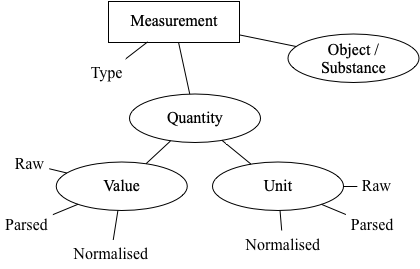
\includegraphics[width=\linewidth]{images/schema-2}
  \caption{Schema of the data model.}
  \label{fig:data-model-schema-2}
  \Description{Schema of the data model.}
\end{figure}

The data model (Figure \ref{fig:data-model-schema-2}) lay its foundation on the concept of \textit{Measurement}, which links an object or a substance with one or more \textit{quantities}. We defined four \textit{Measurements} types: (a) atomic, in case of a single measurement (e.g., 10 grams). (b) interval (\textit{from 3 to 5 km}) and (c) range ($100 \pm 4$ mm) for continuous values, and, (d) a list of discrete values. A \textit{Quantity} links the quantitative value and the unit. 
Since data extracted from PDFs unavoidably present irregular tokens from wrong UTF-8 encoding or missing fonts, we designed this model to allow partial results. The \textit{Value} and \textit{Unit} entities allow three different representations (Figure \ref{fig:data-model-schema-2}): \textit{Raw} as appear in input, \textit{Parsed} unifies the value into the numerical expression, and the unit with its properties (system, type). Finally, \textit{Normalised} contains the transformed unit and values to the SI system. \textit{Value} object supports four types of representations: numeric (2, 1000), alphabetic (two, thousand), scientific notation ($3\cdot10\textsuperscript{5}$), and time, which is also expression of measurements. Units objects are organised following the SI, which allows representing units as products of simpler compounds (e.g. m/s to $m \cdot s\textsuperscript{-1}$) further decomposed as triples (prefix, base and power).

\subsection{Architecture}
The system takes in input text or PDF (the content is extracted in a structured way using the Grobid framework) and performs three steps: (a) tokenisation, (b) measurement extraction and parsing and (c) quantity normalisation. The details of each step are summarised as follows. 

\subsubsection{Tokenisation}
This process splits input data into tokens. Grobid-quantities uses a two-phase tokenisation: (1) first it splits by punctuation marks, then (2) each resulting token is re-tokenised to separate adjacent digits and alphanumeric characters. Given the example \texttt{25m\^{}2}, first returns a list \texttt{[25m, \^{}, 2]} and then recursively divides \texttt{25m} as \texttt{[25, m]}  resulting in \texttt{[25, m, \^{}, 2]}.

\subsubsection{Extraction}
% Quantity model 
The tokens are passed through three ML models, in cascade: first the \textit{Quantities} CRF model determines appropriate unit and value tags. Results are further processed by the respective \textit{Units} and \textit{Values} CRF models as illustrated in Figure \ref{fig:schema-cascade}.  

\begin{figure}[ht]
  \centering
  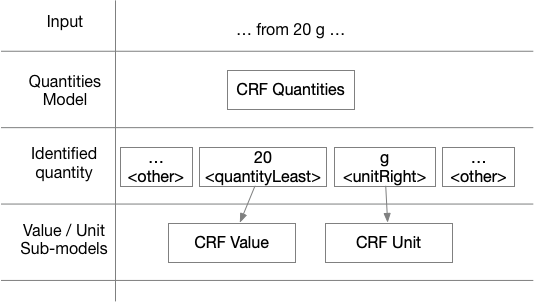
\includegraphics[width=\linewidth]{images/schema-cascade}
  \caption{The cascade approach in applied CRF models. The Quantities model recognises value and units which are passed, respectively, to Values and Units CRF sub-models for further extraction.}
  \label{fig:schema-cascade}
  \Description{The cascade approach in applied CRF models. The Quantities model recognises value and units which are passed, respectively, to Values and Units CRF sub-models for further extraction.}
\end{figure}

Table \ref{tab:quantities-model-labels} describes the labels predicted by the \textit{Quantities} CRF model. Notice that to reconstruct complex structured objects from the flat structure generated by the sequence labelling engine additional labels are necessary (such as <unitLeft>, <unitRight>, for units).

\begin{table}[ht]
  \caption{Labels description for the Quantities CRF model. In bold are highlighted specific examples.}
  \label{tab:quantities-model-labels}
  \begin{tabular}{lll}
    \toprule
    Label & Description & Example\\
    \midrule
    <valueAtomic> & value of an atomic quantity & \textbf{2} m \\
    <valueLeast> & least value in an interval & from \textbf{2} m \\
    <valueMost> & max value in an interval & up to \textbf{7} m \\
    <valueBase> & base value in a range & $\textbf{20}\pm7$ m \\
    <valueRange> & range value in a range & $20 \pm \textbf{7}$ m \\
    <valueList> & list of quantities & \textbf{2}, \textbf{3} and \textbf{10} m \\
    <unitLeft> & left-attached unit & \textbf{pH} 2 \\
    <unitRight> & right-attached unit & 2 \textbf{m} \\
    <other> & everything else & - \\
  \bottomrule
\end{tabular}
\end{table}

% Gazetteers
Previous work (Section \ref{sec:related_work}) presented extensive use of databases or ontologies. In our solution, we used a similar approach. We created a list of units (in English, French and German) with their characteristics: system (SI base, SI derived, imperial, ...) and type (volume, length, ...), and their representations: notations (m\textsuperscript{3}, \texttt{m\^{}3}), lemmas (cubic meter, cubic metre) and inflections (cubic meters, cubic metres). We made this list available through the \textit{Unit Lexicon}, which offers unit lookups by properties (such as notation, lemma, inflexion). A second gazetteer was created to allow the transformation of alphabetic values in numeric ones (for example, twenty-one to 21).

Features in the \textit{Quantities} CRF model are generated from standard information (preceding and following tokens, presence of capital, digits). Orthogonal features are obtained through the \textit{Unit Lexicon}, like a \textit{Boolean} indicating whether a token is a known unit or not. Typographical information (such as format, fonts, subscript and superscript) are ignored. 

% Unit model 
The \textit{Units} CRF model works at character level and uses the \textit{Unit Lexicon} to highlight known units or prefixes. The input tokens are parsed and transformed to a product of triples (prefix, base, power) as shown in Table \ref{tab:units-model-labels}. For example \texttt{Kg/mm\textsuperscript{2}}, corresponds to \texttt{$Kg\cdot mm\textsuperscript{-2}$} and becomes \texttt{[(K, g, 1), (m, m, -2)]} as product of triples. 

\begin{table}[ht]
  \caption{Labels description for the Units CRF model. In bold are highlighted specific examples. }
  \label{tab:units-model-labels}
  \begin{tabular}{lll}
    \toprule
    Label & Description & Example\\
    \midrule
    <prefix> & prefix of the unit  & \textbf{k}m\textsuperscript{2} \\
    <base> & unit base & k\textbf{m}\textsuperscript{2}\\
    <pow> & unit power & km\textsuperscript{\textbf{2}}\\
    <other> & everything else & - \\
  \bottomrule
\end{tabular}
\end{table}

We then use the structured triples to fetch the corresponding information (system, type) from the \textit{Unit Lexicon} and attach them to the resulting object. 
This implementation processes the symbols order from right to left. Priority modifiers, such as parenthesis, are ignored because more complex to manage and not frequent. 

%Let's suppose the raw text contains "10 m 3". The Quantity model identifies 10 as atomic value and "m 3" as the unit. The Unit model identifies "m" as the base and "3" as power: [(,m,3)]. This product is then reformatted as "m\^3" and looked up in the gazetteer. Since "m\^3" exists, system=SI, inflection='Cubic meters' and type=volume are attached to the unit object. 
% Value model 
In parallel, the CRF \textit{Values} model unifies the format of identified values into numerical formats. It supports four types: numeric, alphabetic, scientific notation, and time expression (see Table \ref{tab:values-model-labels}). Different techniques are applied for each type: alphabetic expressions are looked up in the word-to-number gazetteer, scientific notations are parsed and calculated mathematically. Time expressions are further segmented using the Grobid built-in Date CRF model.

\begin{table}[ht]
  \caption{Labels description for the Values CRF model. In bold are highlighted specific examples.}
  \label{tab:values-model-labels}
  \begin{tabular}{lll}
    \toprule
    Label & Description & Example\\
    \midrule
    <number> & numeric value / coefficient & $\textbf{2.5}\cdot10\textsuperscript{\textbf{5}}$ \\
    <alpha> & alphabetic value & \textbf{twenty} \\
    <time> & time expression  & in \textbf{1970-01-02}\\
    <base> & base in scientific notation & $2.5\cdot\textbf{10}\textsuperscript{5}$\\
    <pow> & exponent in scientific notation & $2.5\cdot10\textsuperscript{\textbf{5}}$ \\
    <other> & everything else & - \\
  \bottomrule
\end{tabular}
\end{table}

\subsubsection{Normalisation}

The measurements extracted are transformed to the base SI unit (grams to kg, Celsius to Kelvin, etc.). We used an external Java library called Units of Measurement~\cite{units_of_measurement}, which provides a set of standard interfaces and implementations for safely handling units and quantities. Manipulating measurements with transformations often lead to common mistakes due to wrong rounding and approximations. 
At the time this paper is being written, the final revised version of this library has been accepted under the Java Standardisation Process JSR-385.

\section{Evaluation and results}
\label{sec:results}

We trained and evaluated our system's models using a dataset based on 32 scientific publication (English, Open Access (OA)) and three patents (with translation in English, French and German) randomly selected from different domains such as medicine, robotics, astronomy, and physiology. The training data was generated automatically and then corrected and cross-checked by three annotators. We used 10-fold cross-validation to evaluate each CRF model, independently, and produce precision, recall and f1 scores, as summarised in Table \ref{tab:quantities-evaluation}. 

\begin{table}[ht]
   \caption{Summary of the evaluation scores (precision, recall, F1-score) and label contribution (support) for \textit{Quantities}, \textit{Units} and \textit{Values} CRF models, respectively. }
   \label{tab:quantities-evaluation}
   \begin{tabular}{c|cccc}
        \toprule
        Label & Precision & Recall & F1 & Support\\
        \toprule
        \multicolumn{5}{c}{\textbf{Quantities CRF model}}\\
        \midrule
        <unitLeft>          & 96.76 & 94.71 & 95.71 & 2805  \\
        <unitRight>         & 93.06 & 72.1  & 80.02 & 120   \\
        <valueAtomic>       & 85    & 84.77 & 84.84 & 3599  \\
        <valueBase>         & 78.82 & 76.52 & 77.53 & 94    \\
        <valueLeast>        & 85.05 & 77.39 & 80.94 & 862   \\
        <valueList>         & 72.09 & 54.87 & 61.33 & 494   \\
        <valueMost>         & 84.09 & 73.03 & 78.07 & 878   \\
        <valueRange>        & 84.56 & 81.5  & 82.68 & 93    \\
        all (macro avg.)    & 84.93 & 76.86 & \textbf{80.14}\\
        \midrule
        \multicolumn{5}{c}{\textbf{Unit CRF model}}\\
        \midrule
        <base>              & 99.02 & 99.22 & 99.12 & 3075      \\
        <pow>               & 98.04 & 98.9  & 98.46 & 322       \\
        <prefix>            & 99.19 & 98.8  & 98.99 & 821       \\
        all (macro avg.)    & 98.75 & 98.97 & \textbf{98.86}    \\
        \midrule
        \multicolumn{5}{c}{\textbf{Values CRF model}}\\
        \midrule
        <alpha>             & 96.64  & 98.65 & 97.62  & 826      \\
        <base>              & 83.06  & 69.23 & 72.77  & 58       \\
        <number>            & 98.01  & 99.02 & 98.52  & 3858     \\
        <pow>               & 76.45  & 74.67 & 74.58  & 56       \\
        <time>              & 72.54  & 87.83 & 79.34  & 322      \\
        all (macro avg.)    & 85.34  & 85.88 & \textbf{84.57} & -\\
        \bottomrule
   \end{tabular}
\end{table}

% Scores + discussion Quantities CRF model 
The Quantities CRF model reported an f1 macro average of 80.14\% with precision and recall of 84.93\% and 76.86\%, respectively. The paragraph accuracy was 68.97\%, indicating that more than half of the evaluated paragraphs were correctly labelled. These scores are promising, considering the complexity of the task and the rather small size of the training corpus. In particular \texttt{<list>} and \texttt{<unitRight>} require more example. 

% Scores + discussion Unit CRF model 
The Units CRF model f1 macro average was 98.86\%, with precision and recall reaching 98.75\% and 98.97\%, respectively. Compared with other models, performances were extremely high (more than 10\% for f1 score). 
Such difference can be attributed to (a) the data distribution and (b) the lower variability of unit expressions. We analysed the training data and we noticed that the distribution is biased toward simple units (composed by a single triple). Intuitively, this makes sense, because simple units are statistically more frequent; on the other hand it highlight the necessity of more complex examples. 
Secondly, unit expressions appear, by nature, with lower variability, leading to the generation of more duplicates than in other models' training datasets. For example, the expressions 1\% and 2\% have two different values (1, 2) and the same unit (\%), which would appear twice. 
Since we cannot alter the statistical distribution of the dataset, we can obtain better and more precise measurements of the model generalisation capabilities by using a separate and independent evaluation corpus. 

% Scores + discussion Values CRF model 
The Value CRF model scored average macro f1 at 85.64\% with precision and recall at 81.82\% and 93.29\%, respectively.
We noticed that both \textit{<base>}, \textit{<pow>} and \textit{<time>} have lower f1-score. While \textit{<base>} and \textit{<pow>} require more training data, \textit{<time>} expressions may overlap with \textit{<number>} suggesting more contextual information should be introduced. 


\section{Applications}
\label{sec:use_cases}
Recently, the normalised data extraction is strongly required in materials research. The inverse problem in which high-performance materials are predicted from properties is expected to be solved with well-organised big data. At the National Institute for Materials Science (NIMS), a project to discover new superconducting materials from scientific literature is in progress. The system being developed relies on Grobid-quantities to extract and normalise superconducting properties, such as critical temperature (Tc) with units of mK and K and critical pressure expressed with units of Pa, MPa, and GPa \cite{foppiano2019proposal}. 

Grobid-quantities was showcased in a Text and Data Mining (TDM) platform (within the scope of the French national-wide ISTEX~\cite{dazy2014istex} project) where it provided measurement annotations used to prototype a quantities-based semantic search\footnote{The demo can be accessed at \url{https://traces1.inria.fr/istex_sample/}}. 

Finally, another use was made in a system for extracting semantic measurements and meaning in Earth Science, Marve~\cite{hundman2017measurement}.  

% Istex, Marve, NIMS
\section{Conclusion}
\label{sec:conclusion}
In this paper, we presented Grobid-quantities, a system for extracting and normalising measurement from scientific and patent literature.
The project, the training data and the documentation are accessible on Github\footnote{\url{http://github.com/kermitt2/grobid-quantities}}. 

Results are promising, and the integration in real production platforms proved this application reached a certain level of maturity. Our dataset, although it requires more training examples, is released as open access and can be improved from external contributors. Moreover, as previously discussed, the introduction of an end to end evaluation corpus could provide more objective evaluation results. 

In the future, we plan to introduce recurrent neural networks (RNN) and embeddings for sequence labelling. In particular, contextualised embeddings, trained with values and units could improve the model generalisation. Finally, we plan to integrate domain information and additional layout features (such as superscript/subscripts) to improve unit discrimination. 
 

%%
%% The acknowledgements section is defined using the "acks" environment
%% (and NOT an unnumbered section). This ensures the proper
%% identification of the section in the article metadata, and the
%% consistent spelling of the heading.
\begin{acks}
Our warmest thanks to Patrice Lopez (author of Grobid and many other open-source TDM tools), who initiated and supported Grobid-quantities. Thanks our colleagues at NIMS Thaer M. Dieb, and Akira Suzuki for the support received. Finally, thanks to Units of Measurements's contributors\footnote{\url{https://github.com/orgs/unitsofmeasurement/people}}.
\end{acks}

%%
%% The next two lines define the bibliography style to be used, and
%% the bibliography file.
\bibliographystyle{ACM-Reference-Format}
\bibliography{references}

%%
%% If your work has an appendix, this is the place to put it.
% \appendix

\end{document}
\endinput
%%
%% End of file `sample-sigconf.tex'.
